\section{Einführung}
Stößt ein Elektron auf ein Atom, so unterscheidet man zwischen zwei Arten von Stößen:
\begin{itemize}
	\item Bei \textbf{elastischen} Stößen verliert das Elektron keine Energie, sondern ändert nur die Richtung
	\item Bei \textbf{unelastischen} Stößen wird ein Teil der kinetischen Energie des Elektrons an die am Atom gebundenen Elektronen abgegeben und diese werden in einen höheren Engergiezustand gehoben. Nach kurzer Zeit fallen sie auf das ursprüngliche Niveau zurück, wobei ein Photon ausgesendet wird. Die Energiedifferenz $\Delta E$ hängt über die Plancksche Konstante $h$ mit der Frequenz $\nu$ des ausgesendeten Photons zusammen:
	\begin{equation}
		\Delta E=h\cdot\nu
		\label{eq:deltae}
	\end{equation}
\end{itemize}
Im Franck-Hertz-Versuch werden Elektronen aus einer Glühkathode in einer Triode beschleunigt und stoßen unterwegs mit Gasatomen zusammen. 
Da die Energiezustände der am Elektron gebundenen Atome quantisiert sind und häufig ein bestimmer Energiezustand deutlich wahrscheinlicher ist als andere, muss die kinetische Energie der stoßenden Elektronen diese bestimmte Schwelle $\Delta E$ überschreiten, damit es vermehrt zu unelastischen Stößen kommt. Wird den stoßenden Elektronen kinetische Energie durch eine Beschleunigungsspannung $U_B$ zugeführt, so muss
\begin{equation}
	\Delta E=e\cdot U_B > \Delta E
	\label{eq:energieschwelle}
\end{equation}
gelten.
\begin{figure}[H]
  \centering
  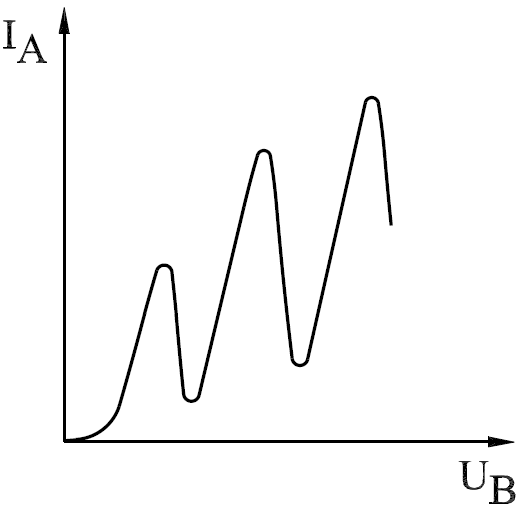
\includegraphics[width=.3\textwidth]{res/theoriekurve}
  \caption{Aus der Theorie erwartete $I_A/U_B$-Charakteristik\footcite{anleitung-ss2015}}
  \label{fig:theoriekurve}
\end{figure}
In \cref{fig:theoriekurve} ist dargestellt, wieviele Elektronen bei einer bestimmten Beschleunigungsspannung die Anode auf der anderen Seite der Triode erreichen. Zunächst ist die Energie der Elektronen zu gering für einen unelastischen Stoß und die Kurve nimmt wie die Kennlinie einer evakuierten Triode zu. Nach dem ersten Maximum ist ein schneller Abfall zu sehen, da hier die kinetische Energie der Elektronen groß genug für einen unelastischen Stoß direkt vor der Anode ist. Nach dem Stoß ist die Restenergie der Elektronen zu gering, um die Anode zu erreichen. Mit höherer Beschleunigungsspannung steigt diese Restenergie und es kommen wieder mehr Elektronen bis zur Anode, bis zum 2. Maxium: ab hier kommt es nun für viele Elektronen zu zwei unelastischen Stößen auf dem Weg durch die Triode usw.\\

Da Quecksilber bei Zimmertemperatur flüssig ist, muss es aufgeheizt werden. Die mittlere freie Weglänge $\lambda$ ist der Erwartungswert der Strecke, die ein Elektron im Gas der Temperatur $T$ und Druck $p$ zurücklegt, bevor es unelastich auf ein Gasatom stößt:
\begin{equation}
	\lambda =\frac{k_B\cdot T}{\sigma \cdot p}
	\label{eq:freierweg}
\end{equation}
Dabei ist der Wirkungsquerschnitt $\sigma$ die Fläche, die ein einfallendes Elektron treffen muss, damit es zum unelastischen Stoß kommt. Bei einem neutralen Atom mit Radius $r$ beträgt $\sigma=\pi r^2$.

Die Clausius-Clapeyron-Gleichung stellt einen Zusammenhang zwischen der Temperatur und dem Dampfdruck eines Gases her. Relevant für den Versuch ist die \textbf{van-t'Hoffsche-Gleichung}, die man durch integrieren der Clausius-Clapeyron-Gl. in der Näherung für ideale Gase erhält\footcite[][342]{dermtroeder}:
\begin{equation}
	p(T)=p_0\cdot e^{\Lambda/R(1/T_0-1/T)}
	\label{eq:clausius}
\end{equation}
Hierbei ist $p_0$ der Dampfdruck zur Temperatur $T_0$, $\Lambda$ die molare Verdampfungswärme des Gases und R die molare Gaskonstante.

\section{Versuch}
\begin{figure}[!htb]
  \centering
  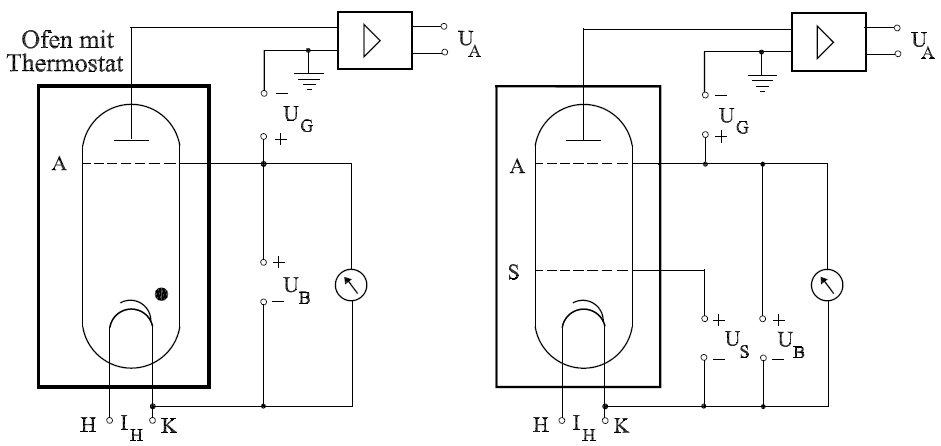
\includegraphics[width=.8\textwidth]{res/aufbau}
  \caption{Aufbau der Franck-Hertz-Röhren mit Quecksilber (links) und Neon (rechts)\footcite{anleitung-ss2015}}
  \label{fig:aufbau}
\end{figure}
Der Aufbau ist in \cref{fig:aufbau} zu sehen. Bei beiden Teilversuchen wird über eine Heizspannung $U_H$ eine Glühkathode in einer Triode zum Glühen gebracht. Eine Beschleunigungsspannung $U_B$ ist zwischen der Glühkathode und einem Gitter in Nähe der Anode auf der anderen Seite der Triode angelegt, sodass aus der Glühkathode austretende Elektronen beschleunigt werden. 

Zwischen diesem Gitter und der Anode ist eine kleine Gegenspannung $U_G$ angelegt, sodass nur Elektronen die Anode erreichen, deren kinetische Energie am Gitter größer als $e\cdot U_G$ ist. 
Der Strom $I_A$ zwischen Anode und Kathode wird über einen Operationsverstärker in eine hierzu proportionale Spannung $U_A$ umgewandelt. Im Folgenden kann mit $U_A$ statt $I_A$ gerechnet werden, da nur die Position der Maxima / Minima der $I_A/U_B$-Kurve entscheidend ist, nicht aber der genauer Wert von $I_A$.

Beim Quecksilberversuch befindet sich die Triode in einem Ofen mit Thermostat, um durch Erhitzen den Quecksilberdampfdruck in der Triode zu erhöhen und damit gemäß \cref{eq:freierweg} die mittlere freie Weglänge der Elektronen zu verringern. Beim Neonversuch ist dies nicht notwendig, da Neon bei Zimmertemperatur schon gasförmig ist. Allerdings befindet sich in der Neontriode zusätzlich ein Streugitter vor der Kathode mit Potentialdifferenz $U_S$, um den Austritt der Elektronen zu vereinfachen.\\

Am Praktikumstag waren die Trioden als fertiges Bauteil mit einem Betriebsgerät bereitgestellt, an dem die Spannungen $U_B$ und $U_G$ sowie die Amplitudenvertärkung durch den Operationsverstärker eingestellt werden konnten. Die Spannungen wurden mit Potentiometern abgelesen.  Zusätzlich konnte am Betriebsgerät die Beschleunigungsspannung auf einen periodischen Sägezahnmodus eingestellt und dann an einem Oszilloskop der $U_A$-Zeit-Verlauf sichtbar gemacht werden.\\

Die Gegenspannung wurde bei allen Versuchen auf $U_G=\SI{1.25(1)}{V}J$ eingestellt.

\subsection{Quecksilbertriode bei Zimmertemperatur}
 Zunächst wurde die $U_A/U_B$-Kurve der Quecksilbertriode bei Zimmertemperatur gemessen. Es wird ein monotoner Anstieg von $U_A$ erwartet, da der Quecksilberdampfdruck sehr niedrig ist und fast keine Stöße stattfinden sollten. Das Ergebnis der Messung ist in \cref{fig:zimmertemp} zu sehen:
\begin{figure}[H]
\centering
\begin{tikzpicture}
  \begin{axis}[
    width=15 cm,
    height=9 cm,
    xmin=-1, xmax=94,
    ymin=-1, ymax=12.5,
    xlabel={Beschleunigungsspannung $U_B$ [\si{V}]},
    ylabel={Anodenspannung $U_A$ [\si{V}]},
    domain=-3:17,
    legend entries={Quecksilbertriode bei Zimmertemperatur},
    legend pos=north west
  ]
  \addplot+ plot [only marks,mark=x, error bars/.cd, x dir=both, x fixed=0.1, y dir=both, y fixed=0.05]  table[skip first n=3, x index=1, y index=0] {res/Q-ZimmerTemp.txt};
  \end{axis}
\end{tikzpicture}
\caption{$U_A/U_B$-Charakteristik der Quecksilbertriode bei Zimmertemperatur}
\label{fig:zimmertemp}
\end{figure}
Die Fehlerbalken sind sehr kurz und deshalb schwer zu erkennen.
Im Bereich von 0 bis \SI{22}{V} Beschleunigungsspannung wurden keine Messwerte aufgenommen, da hier die Anodenspannung fast konstant blieb. Ein näherungsweise linearer Zusammenhang ist für $\SI{0}{V}\leq U_B\leq \SI{60}{V}$ zu erkennen, für höhere Beschleunigungsspannung bleibt die Anodenspannung konstant bei $\SI{11.9}{V}$.

\subsection{Erhitzte Quecksilbertriode}
Die Quecksilbertriode wurde mithilfe des Ofens auf $T=\SI{200(12)}{\degreeCelsius}$ erhitzt. Der Fehler entsteht dadurch, dass der Ofen die Zieltemperatur durch Ein/Aus-Zyklen ansteuert. Es wird ein Verlauf wie in \cref{fig:theoriekurve} erwartet. Die gemessene $U_A/U_B$-Charakteristik ist in \cref{fig:queckheiss} zu sehen:

\begin{figure}[H]
\centering
\begin{tikzpicture}
  \begin{axis}[
    width=15 cm,
    height=9 cm,
    xmin=29, xmax=56.5,
    ymin=-1.5, ymax=12,
    xlabel={Beschleunigungsspannung $U_B$ [\si{V}]},
    ylabel={Anodenspannung $U_A$ [\si{V}]},
    domain=-3:17,
    legend entries={Erhitzte Quecksilbertriode},
    legend pos=north west
  ]
  \addplot+ plot [only marks,mark=x, error bars/.cd, x dir=both, x fixed=0.1, y dir=both, y fixed=0.05]  table[skip first n=2, x index=1, y index=0] {res/Qheiss.txt};
  \draw ({axis cs:35.5,0}|-current axis.south) -- ({axis cs:35.5,0}|-current axis.north);
	\draw ({axis cs:40.5,0}|-current axis.south) -- ({axis cs:40.5,0}|-current axis.north);
	\draw ({axis cs:45.3,0}|-current axis.south) -- ({axis cs:45.3,0}|-current axis.north);
	\draw ({axis cs:50.5,0}|-current axis.south) -- ({axis cs:50.5,0}|-current axis.north);
	

	\end{axis}
\end{tikzpicture}
\caption{$U_A/U_B$-Kurve der Quecksilbertriode bei $T=\SI{200}{\degreeCelsius}$}
\label{fig:queckheiss}
\end{figure}
Die ersten zwei Messwerte wurden ausgelassen, um den Graphen zu entzerren. Die Fehlerbalken sind sehr kurz und deshalb schwer zu erkennen. Es sind die aus der Theorie erwarteten Minima und Maxima zu sehen. Die vertikalen Linien wurden ungefähr über die Extremstellen des Graphen gelegt (nach Augenmaß). Nach einer konservativen Schätzung ist der Fehler dieser Methode so groß wie der größere der beiden Abstände zu den Messpunkten links bzw. rechts von der Linie. Die Anregungsenergie berechnet sich aus der Differenz der Beschleunigungsspannung zwischen zwei aufeinander folgenden Maxima: $\Delta E=e\cdot\Delta U_B$
\begin{table}
\centering
\begin{tabular}{c c c}
		n & $U_B$ [\si{V}] beim n-ten Maximum & $\Delta E$ [\si{eV}] zum (n-1)-ten Maximum  \\ \midrule
		1 & \num{35.5(5)} & - \\
		2 & \num{40.5(5)} & \num{5.0(10)} \\
		3 & \num{45.3(5)} & \num{4.8(10)} \\
		4 & \num{50.5(6)} & \num{5.2(12)}
\end{tabular}
\caption{Anregungsenergie berechnet aus den Abständen zwischen zwei Maxima}
\label{tab:anregen}
\end{table}

Der Mittelwert ist $\Delta E=\SI{5.0(6)}{eV}$. Die Frequenz des ausgesendeten Lichtes beträg laut \cref{eq:deltae} $\nu=\Delta E/h=\SI{1.21e15}{Hz}$, was einer Wellenlänge von $\lambda=c/\nu=\SI{248}{nm}$ entspricht. Dieses Licht liegt also um UV-Bereich und ist nicht sichtbar.\\

Der Dampfdruck von Quecksilber beträgt laut\footcite{hill} $p_0=\SI{0.242}{Pa}$ bei $T_0=\SI{20}{\degreeCelsius}$. Die molare Verdampfungswärme ist $\Lambda=\SI{58.2}{kJ/mol}$\footcite{zhang}. Also ist nach \cref{eq:clausius} der Dampfdruck bei \SI{200}{\degreeCelsius}:
\begin{equation}
	p(\SI{200}{\degreeCelsius})=p_0\cdot e^{\Lambda/R(\frac{1}{\SI{20}{\degreeCelsius}}-\frac{1}{\SI{200}{\degreeCelsius}})}=\SI{2130}{Pa}
	\label{eq:dampfdruck}
\end{equation}\\

Der atomare Radius von Quecksilber ist\footcite{slater} $r=\SI{150}{pm}$, also ist die mittere freie Weglänge bei \SI{20}{\degreeCelsius}
\begin{equation}
	\lambda_{20}=\frac{k_B\cdot \SI{20}{\degreeCelsius}}{\pi\cdot (\SI{150}{pm})^2\cdot \SI{0.242}{Pa}}=\SI{23.66}{cm}
	\label{eq:weg20}
\end{equation}

und bei \SI{200}{\degreeCelsius}
\begin{equation}
	\lambda_{200}=\SI{43}{\micro m}\qquad .
	\label{eq:weg200}
\end{equation}

\subsection{Neontriode}
Analog zur Quecksilbertriode wurde die $U_A/U_B$-Charakteristik der Neonröhre durchgemessen:
\begin{figure}[H]
\centering
\begin{tikzpicture}
  \begin{axis}[
    width=15 cm,
    height=9 cm,
    xmin=-1, xmax=88,
    ymin=-1.5, ymax=10,
    xlabel={Beschleunigungsspannung $U_B$ [\si{V}]},
    ylabel={Anodenspannung $U_A$ [\si{V}]},
    domain=-3:17,
    legend entries={Neontriode},
    legend pos=north west
  ]
  \addplot+ plot [only marks,mark=x, error bars/.cd, x dir=both, x fixed=0.1, y dir=both, y fixed=0.4]  table[x index=1, y index=0] {res/neon.txt};
  \draw ({axis cs:20,0}|-current axis.south) -- ({axis cs:20,0}|-current axis.north);
	\draw ({axis cs:37.7,0}|-current axis.south) -- ({axis cs:37.7,0}|-current axis.north);
	\end{axis}
\end{tikzpicture}
\caption{$U_A/U_B$-Charakteristik der Neontriode}
\label{fig:neon}
\end{figure}
Wieder sind die aus der Theorie erwarteten Minima und Maxima zu sehen. Die anhand der eingezeichneten Maxima bestimmte Anregungsenergie beträgt $\Delta E=e\cdot(\SI{37.7(13)}{V}-\SI{20.0(4)}{V})=\SI{17.7(17)}{eV}$. Würde die gesamte Energie an ein ausgesendetes Photon abgegeben werden, so hätte dieses die Frequenz $\nu=\Delta E/h=\SI{4.28e15}{Hz}$, was einer Wellenlänge von $\lambda=c/\nu=\SI{70}{nm}$ entspräche. 

\section{Diskussion}
\subsection{Nr. 1 und 2}
Die $U_A/U_B$-Kurve in \cref{fig:zimmertemp} ist konsistent mit der mittleren freien Weglänge aus \cref{eq:weg20}, da diese größer als die Triodenlänge ist, d.h. es kommt (fast) nicht zu Stößen zwischen Elektronen und Gasatomen. Die Anodenspannung steigt monoton an, weil die Elektronen immer stärker beschleunigt werden und somit immer mehr die Anode erreichen. Ab $U_B=\SI{60}{V}$ bleibt die Anodenspannung konstant, da alle aus der Glühkathode austretenden Elektronen die Anode erreichen.\\

Nach Aufheizen beträgt die mittlere freie Weglänge $\lambda_{200}=\SI{43}{\micro m}$, ist also deutlich kleiner als die Triodenlänge. Ein durch die Triode fliegendes Elektron stößt also mehrmals mit Gasatomen zusammen. An der $U_A/U_B$-Charakteristik in \cref{fig:queckheiss} ist abzulesen, dass diese Stöße nur dann unelastisch sind, wenn die kinetische Energie der Elektronen $\Delta E$ übersteigt. Der Wert $\Delta E=\SI{5.0(6)}{eV}$ deckt sich innerhalb des Fehlers mit dem wahrscheinlichsten Übergang am Quecksilberatom in den 6p-Zustand (\cref{fig:schemata}).
\begin{figure}[!htb]
  \centering
  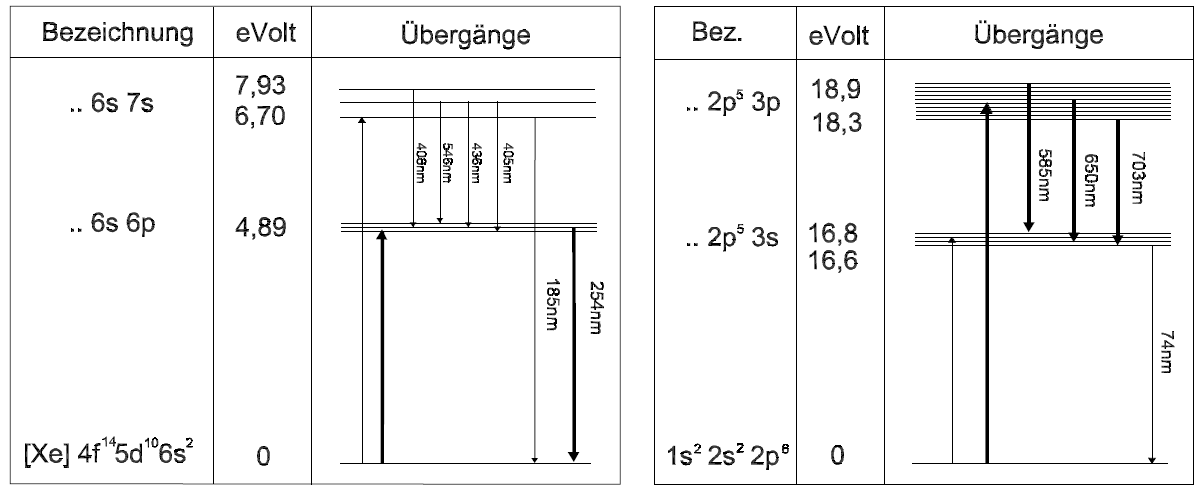
\includegraphics[width=.8\textwidth]{res/schemata}
  \caption{Vereinfachte Termschemata von Quecksilber (links) und Neon(rechts). Dicke Pfeile stellen Übergänge mit der größten Wahrscheinlichkeit dar.\footcite{anleitung-ss2015}}
  \label{fig:schemata}
\end{figure}
\\
Bei der Neonröhre wurden dieselben Beobachtungen gemacht. Auch hier stimmt der gemessene Wert $\Delta E=\SI{17.7(17)}{eV}$ im Rahmen des Fehlers mit dem wahrscheinlichsten Übergang in den 3p-Zustand überein.

\subsection{Nr. 4}
Das emittierte Licht der Neonröhre hat eine Frequenz im sichtbaren Bereich des Lichtes. Dies ist
darauf rückzuführen, dass beim zurück „fallen“ des angeregten Elektron in den Grundzustand,
Photonen mit unterschiedlicher Wellenlänge erzeugt werden, da bei Neon zwischen Zustände
möglich sind. Das Elektron wird in den 3p-Zustand mit einer wahrscheinlichen Anregungsenergie von
18,6eV angeregt. Bei einer vollständigen Abgabe dieser Energie hätte das Photon eine Wellenlänge
von 55,8nm und wäre damit nicht sichtbar. Das Elektron verliert aber seine Energie in zwei Schritten.
Es fällt erst in den 3s-Zustand und anschließend in den Grundzustand. Nach dem Termschemata von
Neon entsteht dadurch auch Licht der Wellenlängen 585nm, 650nm und 703nm. Dieses liegt im
sichtbaren Spektrum des Lichtes. Bei Quecksilber wurden bis auf Leuchterscheinungen die auf der
Glühkathode zurückzuführen sind, keine periodischen Leuchterscheinungen festgestellt. Bei Neon
dagegen schon.

\subsection{Nr. 5}
Bei Quecksilber ist der am wahrscheinlichste angeregte Zustand der 6s 6p Zustand. Unter diesem
liegt nach dem Quecksilber Termschemata keine weiteren Zustände. Das Elektron fällt in den
Grundzustand zurück und die Protonen haben eine Wellenlänge von 185nm oder 254nm. Diese
liegen nicht im Spektrum des Lichtes.

Betrachtet man die Ausgangsspannung der Quecksilberdampflampe bei einer Sägezahn-
Eigenspannung mit einem Oszilloskop so sieht man die typischen Kurvenverläufe der Franck-Hertz-
Röhre. Erhöht man nun die Temperatur der Lampe und damit den Druck so erkennt man am
Oszilloskop, dass die Maxima und Minima weniger stark ausgeprägt sind als bei niedriger Temperatur
oder sogar verschwinden können. Dies kann damit Begründet werden, dass bei hohen Druck mehr
Stoßpartner für die Elektronen vorhanden sind. Damit kommt es zu mehr inelastischen Stößen und
einer größeren Streuung der Elektronen im Raum. Die Maxima und Minima werden dadurch
abgeschwächt.